\begin{surferPage}[משטח מדרגה שישית של בארת']{משטח מדרגה שישית של בארת'}
    משטח זה ממעלה $6$ נוצר על-ידי וולף בארת'
     \textenglish{(Wolf Barth)}
      בשנת 1996.
    
    למשטח של בארת' יש בסך הכל $65$ נקודות סינגולריות.
   זהו המספר המרבי האפשרי של נקודות סינגולריות במשטח מהמעלה השישית, כפי שהוכיחו
    יפה ורוברמן
    
    \textenglish{(Jaffe and Ruberman)} זמן קצר לאחר שבארת' פרסם את המשטח שלו. מכאן,
    שאין אפשרות לשבור את השיא של בארת'!


    משטח זה התקבל בהפתעה גדולה, שכן במשך זמן רב, סברה קהילת המתמטיקאים
    כי משטחים ממעלה $6$ יכולים לכלול רק $64$ נקודות סינגולריות.

   אחת התכונות המעניינות של המבנה הוא סימטריה איקוֹזַהֶדרַלית (סימטריה של עֶשרימוֹן); 
    בתמונה מוצג איקוֹזַהֶדרוֹן (עשרימון) ומישורי הסימטריה שלו:   
  \begin{center}
      \vspace*{-0.1cm}
      \begin{tabular}{@{}c@{\ \ }c@{\,}c@{}}
        \begin{tabular}{@{}c}
          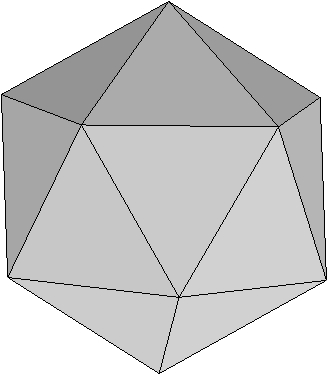
\includegraphics[width=1.4cm]{./../../common/images/icosah}
        \end{tabular}
        &
        \begin{tabular}{@{}c}
          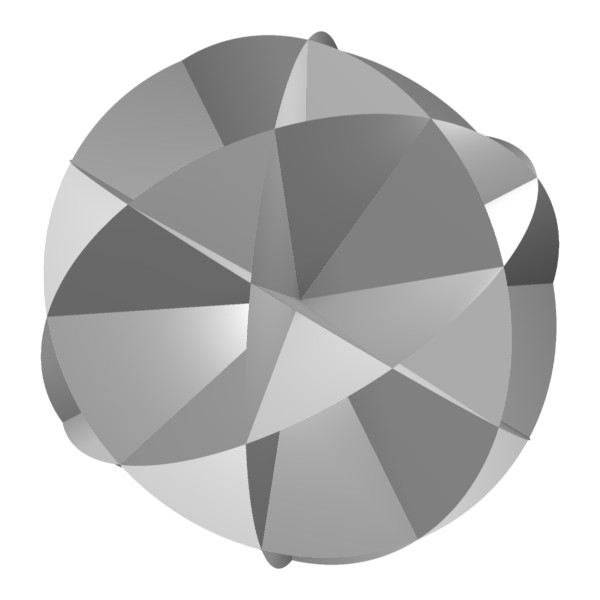
\includegraphics[width=1.4cm]{./../../common/images/barth_sextic_planes}
        \end{tabular}
        &
        \begin{tabular}{c@{}}
          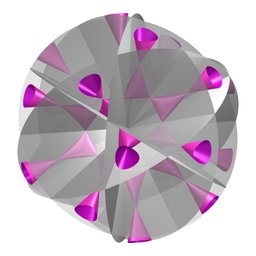
\includegraphics[width=1.4cm]{./../../common/images/barth_sextic_and_planes}
        \end{tabular}
      \end{tabular}
    \end{center}
    \vspace*{-0.1cm}

    המשטח של בארת' מקיים את המשוואה 
    $P_6 - \alpha K^2=0,$ כאשר $P_6$
    מסמל את  
    ששת מישורי הסימטריה, $K=x^2+y^2+z^2-1$ היא סְפֶרַת-היְחִידָה ו- 
    $\alpha=\frac{1}{4}(2+\sqrt{5})$.
\end{surferPage}
